% !TeX root = main.tex
The reference image is shown in Figure \ref{fig:reference}. The data are shown in Figure \ref{fig:data}.

\begin{figure}%
	\centering
	
\includegraphics{plt_demo1_ReferenceImage.eps}	
	
	\caption{Reference Image}\label{fig:reference}
\end{figure}

\begin{figure}%
	\centering
	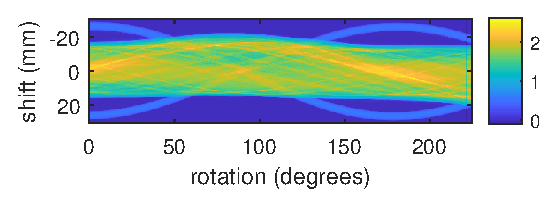
\includegraphics{plt_demo1_Data.eps}	
	
	\caption{Data}\label{fig:data}
\end{figure}

Here are some citations \cite{moon2000,kak2001}.